\documentclass[11pt,a4paper]{article}
\usepackage[margin=2.3cm]{geometry}
\usepackage{amsmath,amssymb,bm}
\usepackage{graphicx}
\usepackage{booktabs}
\usepackage{natbib}
\usepackage[colorlinks=true,linkcolor=blue,citecolor=blue,urlcolor=blue]{hyperref}

\graphicspath{{../../figures/}}
\newcommand{\feh}{\ensuremath{[\mathrm{Fe/H}]}}
\newcommand{\N}{\ensuremath{\mathcal{N}}}

\title{The AstroNN age-error problem in deconvolving the age--metallicity distribution,\\ and a calibration-based solution}
\author{Eos project working note}
\date{26 September 2026}

\begin{document}
\maketitle

\section*{Summary}
\begin{itemize}
  \item Extreme deconvolution (XD) needs, for every star, the distribution of the measured age given the true age, $p(\hat a\mid a)$. Using the AstroNN \texttt{age\_total\_error} as additive Gaussian noise is inconsistent with the data. For high-$\alpha$ giants, the observed age scatter is smaller than the quoted error in every \feh{} bin, with no age-quality cut applied.
  \item With these errors, XD makes the deconvolved density artificially narrow. The convolved model is still broader than the data ($\chi^2/N_{\rm bin}=12.9$).
  \item Rescaling the errors by a fitted factor $s$ fixes the fit ($s\simeq0.3$ in $\ln a$; $\chi^2/N_{\rm bin}=3.8$). The implied error, $\approx9\%$ of the age, is small compared with the width of the distribution, so the deconvolved density is barely narrower than the data.
  \item Rescaling cannot fix the underlying problem. If AstroNN ages are pulled towards the training-set mean, $\hat\ell=\beta\ell+\gamma+\epsilon$ with $\beta<1$, then $\beta$ cannot be determined from the age distribution alone. Any fit to the data recovers the density only up to an unknown stretch of the age axis.
  \item Proposed solution: measure $p(\hat a\mid a,\bm z)$ empirically on asteroseismic ages not used to train AstroNN (APOKASC-3), check it independently with open clusters, and fit XD with that measurement model.
\end{itemize}

\section{Set-up}
We model the joint density of $\bm v=(\ell,\feh)$, where $\ell=\ln(a/{\rm Gyr})$, for the 210{,}355 APOGEE DR17 giants of the Eos base sample \citep{DR17} with a finite, positive AstroNN age \citep{Leung2019,Mackereth2019}. No cut is made on age quality.

XD \citep{Bovy2011} fits
\begin{equation}
p(\bm v)=\sum_{k=1}^{K}\alpha_k\,\N(\bm v\mid\bm\mu_k,\mathbf V_k),\qquad
\hat{\bm y}_i=\mathbf R_i\bm v_i+\bm c_i+\bm\epsilon_i,\quad \bm\epsilon_i\sim\N(\bm 0,\mathbf S_i),
\label{eq:xd}
\end{equation}
by maximising $\sum_i\ln\sum_k\alpha_k\N(\hat{\bm y}_i\mid\mathbf R_i\bm\mu_k+\bm c_i,\ \mathbf R_i\mathbf V_k\mathbf R_i^{\top}+\mathbf S_i)$.

The fits so far use $\mathbf R_i=\mathbf I$ and $\bm c_i=\bm 0$ (additive noise), with $\mathbf S_i=\mathrm{diag}(\sigma_{\ell,i}^2,\sigma_{{\rm Fe},i}^2)$. The \feh{} errors (median 0.009\,dex) are negligible, so the entire problem is in the age dimension.

\section{The problem}

\subsection{Quoted errors exceed the observed scatter}
If $\hat a=a+\epsilon$ with $\epsilon$ independent of $a$, then in any subsample selected without reference to $\hat a$,
\begin{equation}
{\rm Var}(\hat a)={\rm Var}(a)+\langle\sigma^2\rangle\ \ge\ \langle\sigma^2\rangle .
\label{eq:test}
\end{equation}
Figure~\ref{fig:test} and Table~\ref{tab:test} apply this test in \feh{} bins to all finite-age stars.

The test uses no cut on $\sigma_{\rm model}/\hat a$. That cut selects on the measured age and removes 22\% of all stars (48\% at $\feh<-0.6$); applying it would itself create a variance deficit.

\begin{itemize}
  \item With \texttt{age\_total\_error} ($\sigma_{\rm tot}$), eq.~\eqref{eq:test} fails for high-$\alpha$ stars in every bin, and for all stars at $\feh<-0.6$ and $\feh>+0.4$.
  \item With \texttt{age\_model\_error} ($\sigma_{\rm model}$) it holds everywhere.
  \item The DR17 corrected ages give the same signs. Both the linear correction, $(\hat a-0.238)/0.887$ (verified to $1.5\times10^{-6}$ on our sample), and the LOWESS correction (local slope 1.02--1.12) stretch the scatter and the errors alike.
\end{itemize}

\begin{figure}[t]
  \centering
  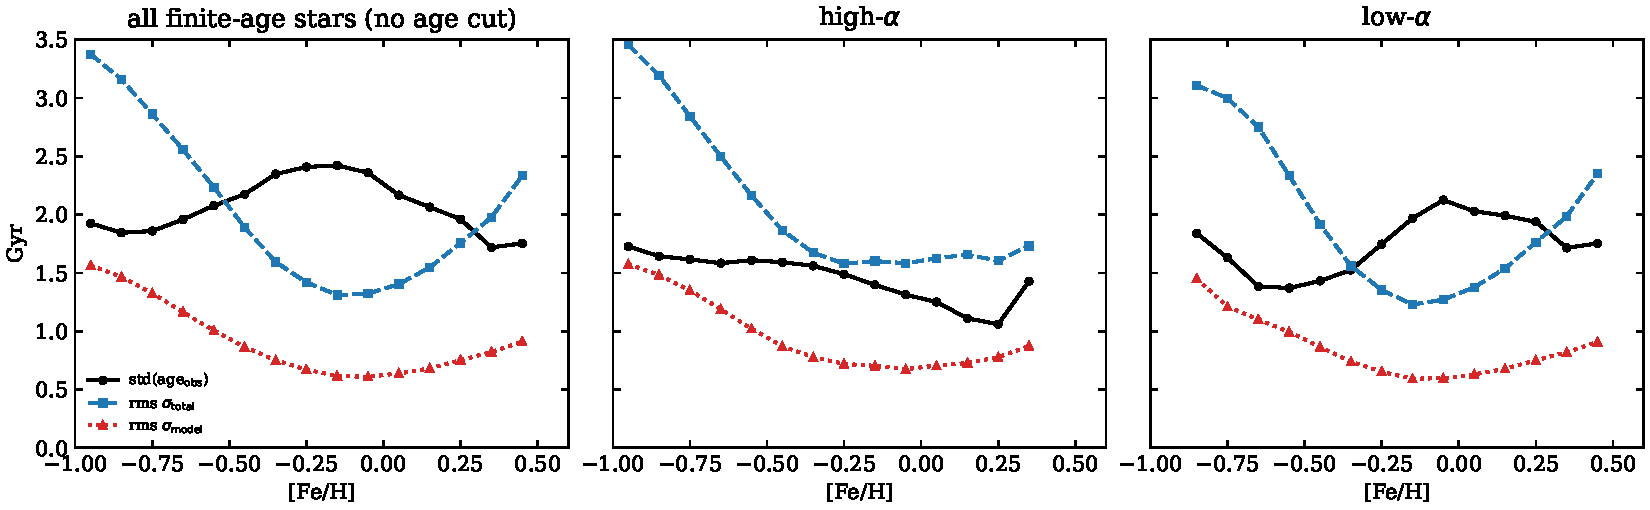
\includegraphics[width=\textwidth]{eos_age_err_consistency_nocut.pdf}
  \caption{Observed scatter of raw AstroNN ages (black) against the rms quoted total (blue) and model (red) errors, in 0.1-dex \feh{} bins, for all finite-age stars. Additive noise requires the black curve to lie above the error curves.}
  \label{fig:test}
\end{figure}

\begin{table}[t]
  \centering\small
  \caption{Test of eq.~\eqref{eq:test}: ${\rm Var}(\hat a)-\langle\sigma^2\rangle$ [Gyr$^2$] for raw ages, all finite-age stars. Negative entries are inconsistent with additive noise.}
  \label{tab:test}
  \begin{tabular}{lrrrr}
    \toprule
    & \multicolumn{2}{c}{all stars} & \multicolumn{2}{c}{high-$\alpha$}\\
    \feh{} & $\sigma_{\rm tot}$ & $\sigma_{\rm model}$ & $\sigma_{\rm tot}$ & $\sigma_{\rm model}$\\
    \midrule
    $-1.0$ to $-0.8$ & $-6.98$ & $+1.26$ & $-7.98$ & $+0.50$\\
    $-0.8$ to $-0.6$ & $-3.38$ & $+2.22$ & $-4.35$ & $+0.99$\\
    $-0.6$ to $-0.4$ & $+0.51$ & $+3.80$ & $-1.49$ & $+1.67$\\
    $-0.4$ to $-0.2$ & $+3.42$ & $+5.19$ & $-0.33$ & $+1.77$\\
    $-0.2$ to $\phantom{+}0.0$ & $+4.00$ & $+5.35$ & $-0.67$ & $+1.39$\\
    $\phantom{+}0.0$ to $+0.2$ & $+2.37$ & $+4.09$ & $-1.22$ & $+0.95$\\
    $+0.2$ to $+0.4$ & $+0.26$ & $+3.00$ & $-1.18$ & $+0.87$\\
    \bottomrule
  \end{tabular}
\end{table}

\subsection{Consequence for XD}
Where $\langle\sigma^2\rangle$ approaches or exceeds ${\rm Var}(\hat a)$, the likelihood is maximised by intrinsic age variances $\mathbf V_k^{aa}\to0$.

The XD fit in linear age with $\sigma_{\rm tot}$ (age-cut sample, $K=20$; Fig.~\ref{fig:compare}, left) therefore shows thin sequences. Even with near-zero intrinsic widths, its convolved model is broader than the data at every \feh{}: the std of age is 1.09 vs 1.49\,Gyr at $\feh=-0.80$ and 2.39 vs 2.63\,Gyr at $\feh=-0.21$ (data vs model), and $\chi^2/N_{\rm bin}=12.9$. The thin sequences are a consequence of the error model, not resolved structure.

\subsection{Rescaling the errors}
We replaced $\sigma_\ell=\sigma_{\rm tot}/\hat a$ by $s\,\sigma_{\rm tot}/\hat a$ and selected $s$, the coordinate ($a$ or $\ln a$) and $K$ by five-fold held-out $\ln p(a,\feh)$, using per-star paired standard errors:
\begin{itemize}
  \item $\ln a$ beats linear $a$ at every $s$, by $0.0186\pm0.0006$ per star at $s=0.4$.
  \item At $K=12$, the score falls away from $s\simeq0.25$--0.4: by $-0.0019\pm0.0003$ at $s=0.2$, $-0.0013\pm0.0001$ at $s=0.5$ and $-0.056$ at $s=1$.
  \item Over $s\in\{0.25,0.3,0.4\}$ and $K\le28$, the best is $s=0.30$, $K=28$. The score is still rising slowly at $K=28$ ($3\times10^{-4}$ per star from $K=24$).
\end{itemize}
The full-sample fit at $s=0.30$, $K=28$ (Fig.~\ref{fig:compare}, right) has $\chi^2/N_{\rm bin}=3.8$, and its three random starts agree to $2\times10^{-5}$ per star.

\begin{figure}[t]
  \centering
  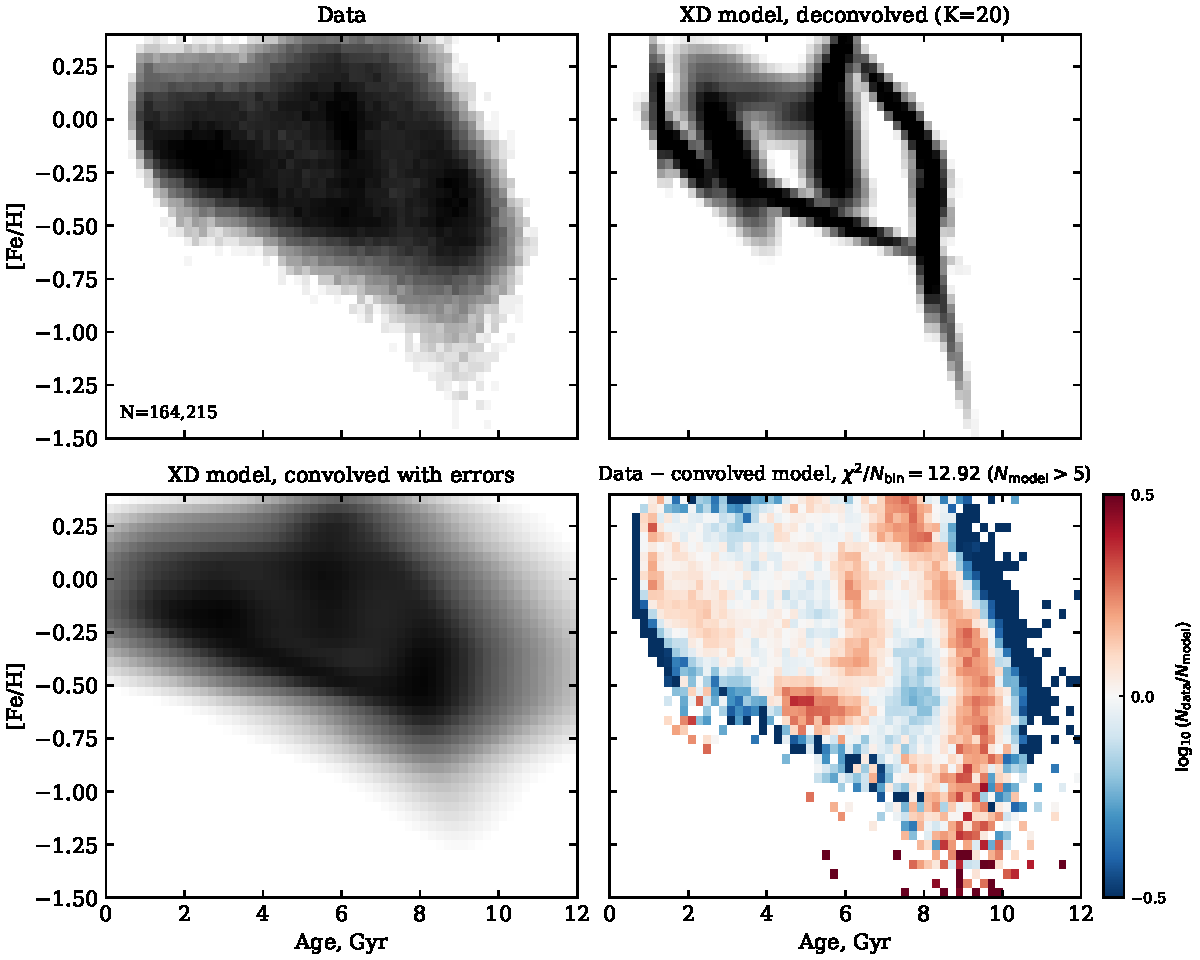
\includegraphics[width=0.49\textwidth]{eos_age_feh_xd.pdf}\hfill
  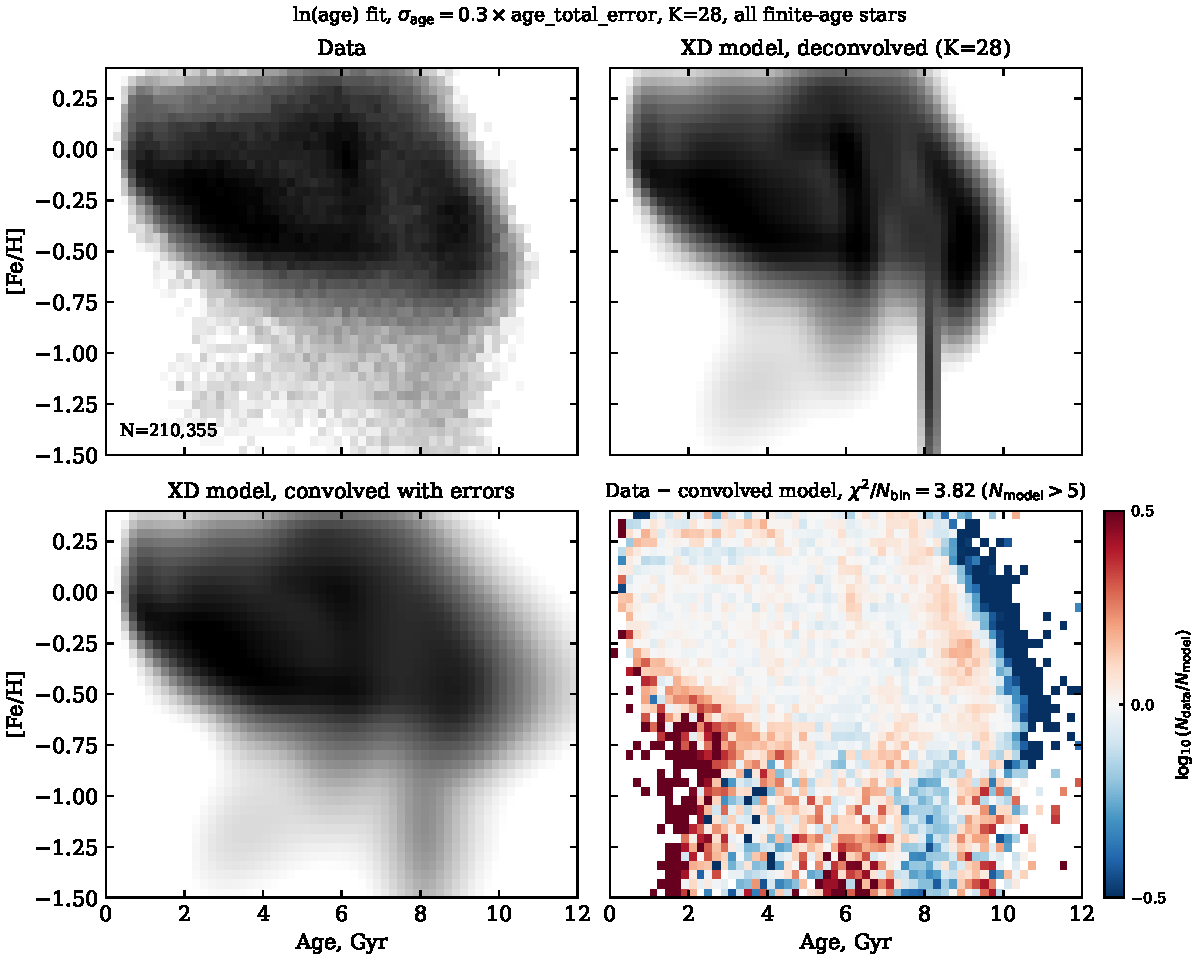
\includegraphics[width=0.49\textwidth]{eos_age_feh_xd_best.pdf}
  \caption{\emph{Left:} XD with $\sigma_{\rm tot}$ as additive noise (linear age, age-cut sample, $K=20$). \emph{Right:} XD with rescaled errors ($\ln a$, $s=0.30$, all finite-age stars, $K=28$). Panels in each: data, deconvolved model, convolved model, $\log_{10}$(data/convolved model).}
  \label{fig:compare}
\end{figure}

Its deconvolved density is only slightly narrower than the data, because the fitted error is small compared with the spread of ages (Table~\ref{tab:narrow}).

\begin{table}[t]
  \centering\small
  \caption{Spread of $\ln\hat a$ in \feh{} rows, rms noise $\sigma_\ell$, and the implied narrowing $1-\sqrt{{\rm Var}(\hat\ell)-\langle\sigma_\ell^2\rangle}/{\rm std}(\hat\ell)$, for $s=1$ and $s=0.3$. The median $\sigma_\ell$ is 0.297 for $s=1$ and 0.089 for $s=0.3$.}
  \label{tab:narrow}
  \begin{tabular}{lrrrrr}
    \toprule
    \feh{} & std$(\hat\ell)$ & $\sigma_\ell$ ($s=1$) & narrowing & $\sigma_\ell$ ($s=0.3$) & narrowing\\
    \midrule
    $-0.9$ to $-0.7$ & 0.309 & 0.481 & 100\% & 0.144 & 12\%\\
    $-0.6$ to $-0.4$ & 0.400 & 0.405 & 100\% & 0.122 & 5\%\\
    $-0.3$ to $-0.1$ & 0.596 & 0.319 & 16\% & 0.096 & 1\%\\
    $\phantom{+}0.0$ to $+0.2$ & 0.598 & 0.302 & 14\% & 0.091 & 1\%\\
    \bottomrule
  \end{tabular}
\end{table}

\subsection{Why rescaling is not a solution}
\label{sec:degeneracy}
\paragraph{The AstroNN error is not the error XD needs.}
AstroNN's \texttt{total} uncertainty is the width of its predictive distribution, combining a learned aleatoric variance and dropout model variance \citep{Leung2019}. XD needs the scatter of the estimate about the truth, ${\rm Var}(\hat a-a\mid a)$. The two need not agree.

\paragraph{AstroNN ages are probably pulled towards the mean.}
A network regressing on training ages \citep[APOKASC-2;][]{Pinsonneault2018} behaves like a posterior mean. Its estimates are under-dispersed: ${\rm Var}(\hat a)={\rm Var}(a)-{\rm E}[{\rm Var}(a\mid{\rm data})]$. A linear model of this is
\begin{equation}
\hat\ell=\beta\ell+\gamma+\epsilon,\qquad\epsilon\sim\N(0,\tau^2),\qquad\beta<1 .
\label{eq:shrink}
\end{equation}
Three observations fit this picture:
\begin{itemize}
  \item the DR17 linear correction has slope $0.887<1$ in $\hat a$;
  \item only 0.5\% of raw ages exceed 10\,Gyr, with a sharp fall-off above 9.5\,Gyr;
  \item the variance deficit is largest where training stars are scarce (old, metal-poor).
\end{itemize}

\paragraph{$\beta$ cannot be determined from the data alone.}
Under eq.~\eqref{eq:shrink} the observed density depends on $\ell$ only through $u=\beta\ell+\gamma$:
\[
p(\hat\ell)=\int\N(\hat\ell\mid u,\tau^2)\,f_u(u)\,du .
\]
Any $(\beta,\gamma)$ paired with the corresponding stretched $f(\ell)$ gives the same likelihood. Fitting $s$ with $\mathbf R_i=\mathbf I$ implicitly sets $\beta=1$ and returns $f_u$: the density on the AstroNN age scale, not the true-age scale.

If $\beta<1$, the true density is \emph{wider} than the right panel of Fig.~\ref{fig:compare} by a factor $1/\beta$ in $\ell$. Structure near the age ceiling, such as the vertical band at $\hat a\approx8.2$\,Gyr for $\feh<-1$, may be compressed older ages. Only stars with independently known ages can determine $\beta$, $\gamma$ and $\tau$.

\section{Proposed solution}

\subsection{Measurement model}
Measure the kernel
\begin{equation}
\hat\ell=m(\ell,\bm z)+\epsilon,\qquad \epsilon\sim\N\!\left(0,\tau^2(\bm z)\right),
\label{eq:kernel}
\end{equation}
with $m$ a monotonic low-order spline in $\ell$. The observables $\bm z$ are, in order of priority: evolutionary state (RGB/RC), \feh, [$\alpha$/Fe], $\log g$, S/N. The linear form of eq.~\eqref{eq:shrink} is the special case $m=\beta(\bm z)\ell+\gamma(\bm z)$. It is adopted only if it describes the calibration stars as well as the spline does on held-out data.

\subsection{Calibration sample}
\begin{itemize}
  \item \textbf{Stars:} APOKASC-3 \citep{Pinsonneault2025}, about 12{,}400 evolved stars with asteroseismic ages, cross-matched with our catalogue.
  \item \textbf{Leakage:} exclude stars used to train AstroNN. At minimum this means APOKASC-2 \citep{Pinsonneault2018} members; better, the actual training list, if it can be obtained.
  \item \textbf{Fit:} maximum likelihood with seismic age errors included, since the calibration is itself an errors-in-variables problem.
  \item \textbf{Validate on held-out calibration stars:}
    \begin{enumerate}
      \item the distribution of standardised residuals $(\hat\ell-m)/\tau$;
      \item whether the quoted AstroNN intervals achieve their nominal coverage;
      \item trends of the residuals with $\ell$ and each $z$.
    \end{enumerate}
  \item \textbf{Coverage:} report where the calibration sample covers the (age, \feh) plane. Outside that region the model extrapolates and must be flagged.
\end{itemize}

\subsection{Independent check with open clusters}
Members of an open cluster share one true age. In APOGEE DR17 open-cluster members \citep{Myers2022}:
\begin{itemize}
  \item the within-cluster spread of $\hat\ell$ measures $\tau$ directly;
  \item the cluster mean against the literature age measures $m(\ell)$ and any pull towards the mean, including at old ages.
\end{itemize}
Clusters are not needed to fit eq.~\eqref{eq:kernel}; they test it.

\subsection{Deconvolution with the measured kernel}
\begin{itemize}
  \item \textbf{Linear $m$:} eq.~\eqref{eq:xd} with $\mathbf R_i=\mathrm{diag}(\beta(\bm z_i),1)$, $\bm c_i=(\gamma(\bm z_i),0)$ and $\mathbf S_i=\mathrm{diag}(\tau^2(\bm z_i),\sigma^2_{{\rm Fe},i})$ is exact projection XD. The existing 2D element-wise code extends directly.
  \item \textbf{Non-linear $m$ depending only on $(\ell,\feh)$:} fit additive-noise XD in $(u,\feh)$ with $u=m(\ell,\feh)$ and noise $\tau$. Then transform back:
    \[f(\ell,\feh)=g\big(m(\ell,\feh),\feh\big)\,|\partial m/\partial\ell| .\]
  \item \textbf{Dependence on $\bm z$ outside the model coordinates (e.g.\ evolutionary state):} linearise $m$ about each star's estimate to get per-star $\mathbf R_i$ and $\bm c_i$. Check the approximation by injection--recovery.
  \item \textbf{Sample:} no cut on $\hat a$ or $\sigma/\hat a$; stars with poor ages simply carry little weight. If a cut is required, its selection function enters the likelihood.
  \item \textbf{Age limit:} support is truncated at $a=13.8$\,Gyr if the fitted mass above it exceeds 1\%.
\end{itemize}

\subsection{Validation and resolution}
Draw mock stars from known intrinsic densities, pass them through the measured kernel and the same selection, and refit. The mocks are: a three-population Galactic model (broad low-$\alpha$ disc, narrow tilted high-$\alpha$ sequence, old metal-poor tail), and single features of varying age width. This gives:
\begin{enumerate}
  \item the bias of the recovered density;
  \item a resolution curve: the smallest feature width recoverable at each (age, \feh);
  \item the size of artefacts produced by the current additive-noise model on the same mocks.
\end{enumerate}
Model selection keeps five-fold held-out likelihood with paired standard errors, together with data$-$model residual maps.

\subsection{Order of work and acceptance tests}
\begin{enumerate}
  \item \textbf{Calibration.} Obtain APOKASC-3, cross-match, remove training stars, plot $\hat\ell$ against $\ell_{\rm seis}$.
    \emph{Test:} fitted $\beta$ with its uncertainty; standardised residuals of unit variance on held-out stars.
  \item \textbf{Kernel choice.} Fit the spline and linear kernels.
    \emph{Test:} held-out likelihood of calibration stars; with the fitted kernel, the variance test $\mathrm{Var}(\hat\ell)\ge\langle\tau^2\rangle$ holds in every \feh{} bin.
  \item \textbf{Cluster check.} \emph{Test:} within-cluster scatter consistent with $\tau$; cluster means consistent with $m$.
  \item \textbf{Deconvolution.} Projection XD on the full sample; injection--recovery.
    \emph{Test:} $\chi^2/N_{\rm bin}$ at least as good as the $s=0.3$ fit; mock densities recovered within the resolution curve.
\end{enumerate}

\begin{thebibliography}{99}
\bibitem[Abdurro'uf et al.(2022)]{DR17} Abdurro'uf et al., 2022, ApJS, 259, 35. \href{https://doi.org/10.3847/1538-4365/ac4414}{doi:10.3847/1538-4365/ac4414}, \href{https://arxiv.org/abs/2112.02026}{arXiv:2112.02026}.
\bibitem[Bovy et al.(2011)]{Bovy2011} Bovy J., Hogg D.~W., Roweis S.~T., 2011, Ann. Appl. Stat., 5, 1657. \href{https://doi.org/10.1214/10-AOAS439}{doi:10.1214/10-AOAS439}, \href{https://arxiv.org/abs/0905.2979}{arXiv:0905.2979}.
\bibitem[Leung \& Bovy(2019)]{Leung2019} Leung H.~W., Bovy J., 2019, MNRAS, 483, 3255. \href{https://doi.org/10.1093/mnras/sty3217}{doi:10.1093/mnras/sty3217}, \href{https://arxiv.org/abs/1808.04428}{arXiv:1808.04428}.
\bibitem[Mackereth et al.(2019)]{Mackereth2019} Mackereth J.~T. et al., 2019, MNRAS, 489, 176. \href{https://doi.org/10.1093/mnras/stz1521}{doi:10.1093/mnras/stz1521}, \href{https://arxiv.org/abs/1901.04502}{arXiv:1901.04502}.
\bibitem[Myers et al.(2022)]{Myers2022} Myers N. et al., 2022, AJ, 164, 85, \emph{OCCAM VI: Galactic chemical gradient analysis from APOGEE DR17}. \href{https://doi.org/10.3847/1538-3881/ac7ce5}{doi:10.3847/1538-3881/ac7ce5}, \href{https://arxiv.org/abs/2206.13650}{arXiv:2206.13650}.
\bibitem[Pinsonneault et al.(2018)]{Pinsonneault2018} Pinsonneault M.~H. et al., 2018, ApJS, 239, 32. \href{https://doi.org/10.3847/1538-4365/aaebfd}{doi:10.3847/1538-4365/aaebfd}, \href{https://arxiv.org/abs/1804.09983}{arXiv:1804.09983}.
\bibitem[Pinsonneault et al.(2025)]{Pinsonneault2025} Pinsonneault M.~H. et al., 2025, ApJS, 276, 69. \href{https://doi.org/10.3847/1538-4365/ad9fef}{doi:10.3847/1538-4365/ad9fef}, \href{https://arxiv.org/abs/2410.00102}{arXiv:2410.00102}.
\end{thebibliography}
\end{document}
